% ........................................................................... %

\chapter{Semantics of protocol timed automata}
\label{chap:pta-semantics}

% ........................................................................... %

The semantics of protocol timed automata over an infinite labeled transition system $\mathcal{S}_A$ are borrowed from those of event-clock automata \cite{RALF94}, another class of timed automata defined over $\T = \Rpos \cup \{ \perp \}$.

\begin{definition}[Protocol timed automata semantics]
The semantic of a protocol timed automaton $A = (L, L^0, L^f, X \cup Y, E, \Sigma)$ is given by the (infinite) LTS $\mathcal{S}_A = (S, s_0, \rightarrow, \Sigma)$ where:
\begin{itemize}

    \item $S = L \times \T^X$ is the set of states $(l, v)$ (also called \emph{configurations}) comprising each a location and a clocks valuation,

    \item $s_0 = (l_0, v_0)$ with $l_0 \in L^0$ and $v_0(x) = \perp$ $\forall x \in X$,

    \item $\rightarrow$ is the transition relation:
    \begin{itemize}

        \item action transitions: $(l, v) \stackrel{a}{\longrightarrow} (l', v')$ if and only if there exists
        $e = (l, g, a, r, l') \in E$ such that $v \models g$, $v' = [r \leftarrow 0]v$ 

        \item time transitions: $\stackrel{d}{\longrightarrow} (l, v')$ for $d \in \Rpos$ if $\forall x \in X$:
        \begin{itemize}
          \item if $v(x) \neq \perp$ then $v'(x) = v(x) + d$, else
          \item if $v(x) = \perp$ then $v'(x) = \perp$.
        \end{itemize}

    \end{itemize}

\end{itemize}
\end{definition}

A timed word $w$ is recognized by a protocol timed automaton $A$ if there exists a run over $\mathcal{S}_A$: $(l_0, v_0) \stackrel{d_0}{\longrightarrow} (l_0, v_1) \stackrel{a}{\longrightarrow} (l_1, v_1) \stackrel{\cdots}{\longrightarrow} \cdots \stackrel{\cdots}{\longrightarrow} (l_n, v_n)$ such that $l_n \in L^F$.\\

Reachability analysis is the key to most of the analysis techniques on timed automata. The formal grounds for this reside in the ability to group ``similar'' configurations that each comprise the current location and a clocks valuation. Those groups, called regions, are built using an equivalence relation between the configurations that represent the states of the (infinite) labeled transition system associated to a timed automaton \cite{RADLD94}. We adapt an equivalence relation for protocol timed automata.\\

We define an equivalence relation between the states of $\mathcal{S}_A$, denoted as $\cong$. We denote the integer part of a real-valued number $r \in \Rpos$ as $\lfloor r \rfloor$ and its fractional part as $\{ r \}$ (e.g., $\lfloor 2.55 \rfloor = 2$ and $\{ 2.55 \} = 0.55$).

\begin{definition}
Two configurations $(l, v)$ and $(l', v')$ are \emph{equivalent}, denoted as $(l, v) \cong (l', v')$ if $l = l'$ and:
\begin{enumerate}
  
  \item $\forall x \in X$:
  \begin{itemize}
    \item if $v(x) = \perp$ then $v'(x) = \perp$, else
    \item $\lfloor v(x) \rfloor = \lfloor v'(x) \rfloor$ or both $v(x) > c_x$ and $v'(x) > c_x$
  \end{itemize}
  
   \item $\forall x,y \in X$ such as $v(x) \leq c_x$ and $v(y) \leq c_y$, then $\{v(x)\} \leq \{v(y)\}$ if and only if $\{v'(x)\} \leq \{v'(y)\}$

  \item $\forall x \in X$ such as $v(x) \leq c_x$, $\{v(x)\} = 0$ if and only if $\{v(x)\} = 0$.
  
\end{enumerate}
\end{definition}

% ........................................................................... %

\chapter{An overview of UPPAAL}
\label{chap:uppaal}

% ........................................................................... %

We present here the model used in UPPAAL which is based on timed automata. Then, we present the query language of UPPAAL before finishing with the tools that it provides.

% ........................................................................... %

\section{UPPAAL model and query language}

% ........................................................................... %

UPPAAL uses an hybrid extension of timed automata as a model and a subset of TCTL as a query language to express properties. Briefly, an hybrid system \cite{alur97symbolic} features both continuous (e.g., variables in $\R$) and discrete behavior (e.g., variables in $\N$). This allows mixing discrete variables such as booleans or integers with clocks in the models that are processed by UPPAAL. Those discrete variables can be used in guards, invariants and be reset on switches just like a clock would be. Actually, a timed automaton can be viewed as a linear hybrid automaton whose continuous variables evolve at a constant rate \cite{alur97symbolic}. Further pointers on hybrid automata can be found in \cite{Miller00, HYTECH, ACHH93}. \\

\begin{figure}[htbp]
    \centering
    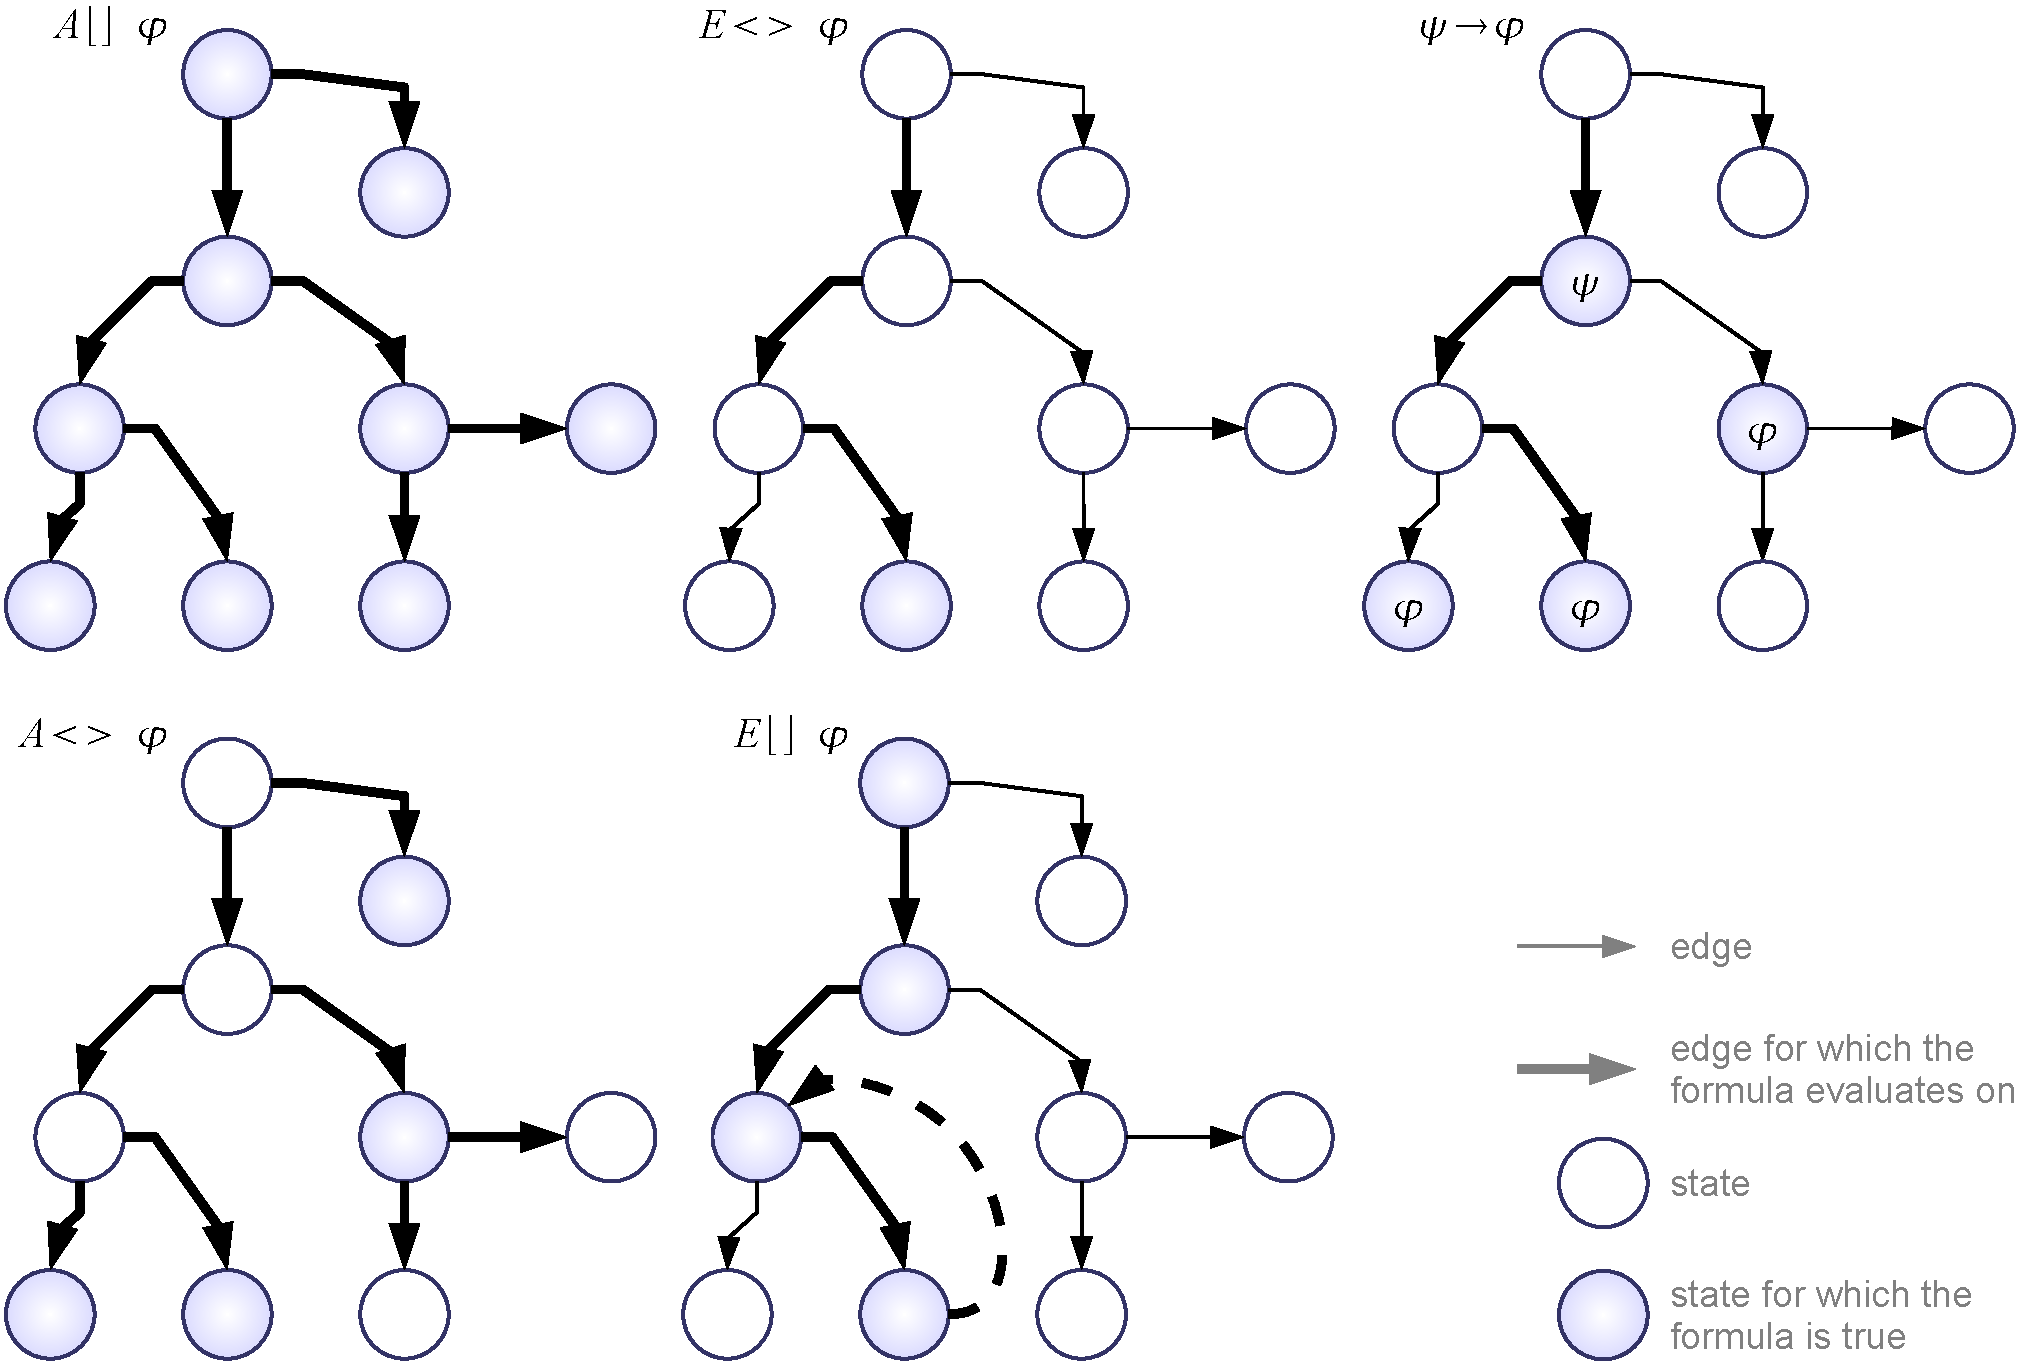
\includegraphics[width=\textwidth]{content/timed-automata/uppaal-path-formulae}
    \begin{flushright}
    	\textit{(source: \cite{UPPAAL})}
    \end{flushright}
    \caption{The path formulae that UPPAAL supports.}
    \label{fig:uppaal-path-formulae}
\end{figure}

We summarize here the types of formula that can be defined for queries in UPPAAL as detailed in \cite{UPPAAL}. We will use Figure~\ref{fig:uppaal-path-formulae} to illustrate them. To begin with, we need \emph{state formula}. Such a formula can be made from clock constraints (e.g., $(x < 3.75) \wedge (y \geq 5)$) and tests that check if a system is in a given location or not (e.g., $P.l$ is true when the system $P$ is currently in the $l$ location). By combining them using boolean conjunctions and disjunctions, it is possible to define complex state formulae such as $\varphi = (x < 3.75) \wedge (y \geq 5) \wedge P.l$. There is also a special state formula $\mathtt{deadlock}$ that is true when neither the current extended state $(l, v)$ offers an outgoing action transition nor there exists a time successor $(l, v')$ that does so. Using state formulae as a basis, the path formulae that can be expressed have been summarized in Table~\ref{tab:uppaal-path-formulae}.\\

\begin{table}[htbp]
\footnotesize
\centering
\begin{tabular}{|p{3cm}|p{7cm}|p{2cm}|}
  
  \hline
  
  \textit{Formula} &
  \textit{Semantic} &
  \textit{Analysis} \\
  
  \hline
  
  $E\Diamond \varphi$ &
  There exists a path to a state $(l, v)$ that verifies $\varphi$. &
  Reachability \\
  
  \hline
  
  $A\Box \varphi$ &
  Every reachable state $(l, v)$ satisfies $\varphi$. &
  Safety \\
  
  \hline
  
  $E\Box \varphi$ &
  There exists a path to a state $(l, v)$ with no outgoing transition that satisfies $\varphi$, or there exists an infinite path where $\varphi$ is satisfied by all states at some point. &
  Safety \\
  
  \hline
  
  $A\Diamond \varphi$ &
  For every possible path, there exists a state $(l, v)$ such that $\varphi$ is satisfied. &
  Liveness \\
  
  \hline
  
  $\varphi \rightarrow \psi$, or equivalently $A\Box (\varphi \Rightarrow A\Diamond \psi)$ &
  Given a state $(l_1, v_1)$ satisfying $\varphi$, every path starting from it contains a state $(l_2, v_2)$ such that $\psi$ is satisfied. &
  Liveness \\
  
  \hline
  
\end{tabular}
\caption{Semantics of the path formulae supported by UPPAAL (a subset of TCTL).}
\label{tab:uppaal-path-formulae}
\end{table}

Going back to the examples of verifications that we expressed as \emph{property 1} and \emph{property 2} on Figure~\ref{fig:light-verification-inclusion}, the properties can be checked by UPPAAL using the following formulae:
\begin{itemize}
  
  \item \emph{property 1}: $E\Diamond (\mathsf{Model.off \wedge x = 10})$ (the location $\mathsf{Model.off}$ is reachable while the clock $x$ has a valuation of 10)
  
  \item \emph{property 2}: $E\Diamond (\mathsf{Model.off \wedge x = 1})$ (there is a path to a state in the LTS of $\mathsf{Model}$ such that the current location is $\mathsf{Model.off}$ and the current valuation of the clock $x$ is 1).
  
\end{itemize}
UPPAAL evaluates the first property to \texttt{true} and the second one to \texttt{false}. Please note that ``undesirable'' properties (i.e., the ones that should normally evaluate to \texttt{false}) are expressed \emph{positively} in UPPAAL (as opposed to \emph{negatively} using a boolean negation operator).\\

UPPAAL supports a subset of TCTL. which provides more path formulae. Also, TCTL allows nested path formulae, something that UPPAAL does not support.

% ........................................................................... %

\section{UPPAAL tools}

% ........................................................................... %

\begin{figure}[htbp]
    \centering
    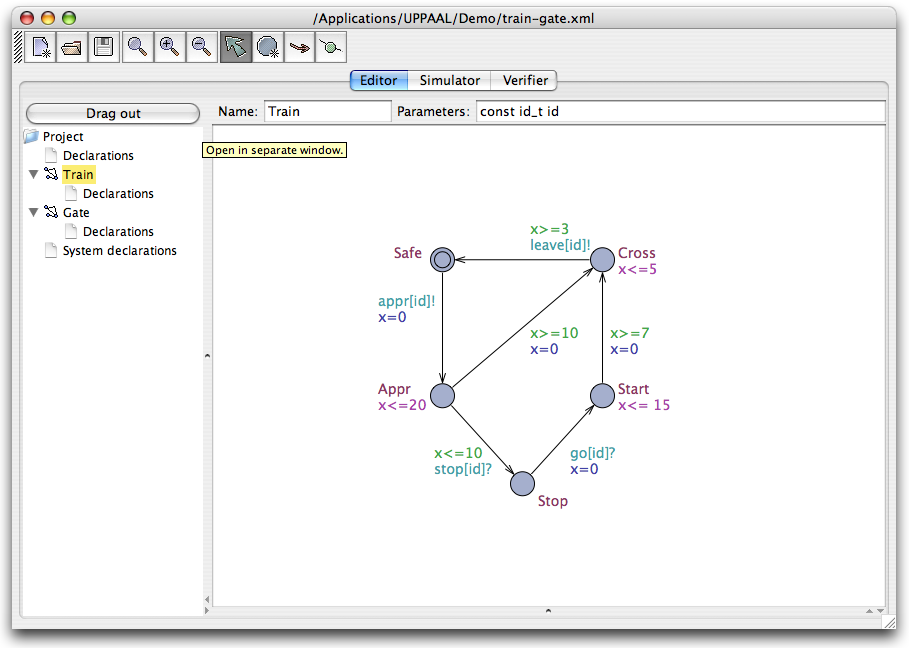
\includegraphics[width=\textwidth]{content/timed-automata/uppaal-1}
    \caption{UPPAAL: modeling environment.}
    \label{fig:uppaal-1}
\end{figure}

UPPAAL comprises two main components:
\begin{enumerate}
  
  \item a command-line model checker called \emph{verifyta}, written in C and ported to Unix variants (Linux, *BSD), Windows and Mac OS X, and
  
  \item a graphical user interface (GUI) written in Java.
  
\end{enumerate}
The UPPAAL GUI (see Figure~\ref{fig:uppaal-1}) is a comprehensive environment for modeling, simulating and verifying systems represented as timed automata. The editor allows to define a set of (usually interacting) systems (e.g., the gate, barrier controller and train systems of the examples found in \cite{RADLD94} or the light controller of Figure~\ref{fig:light-verification-inclusion}).\\

\begin{figure}[htbp]
    \centering
    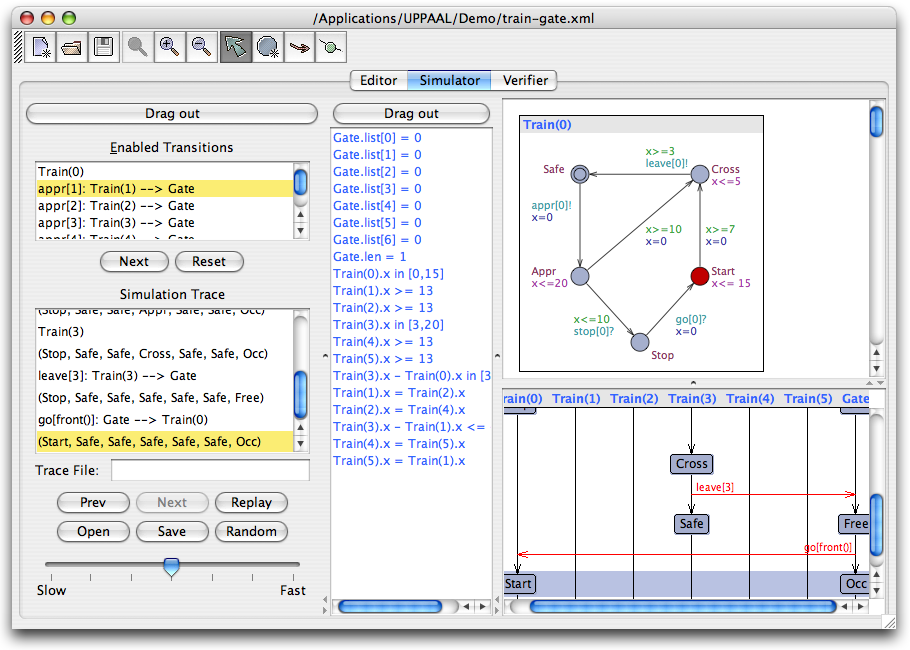
\includegraphics[width=\textwidth]{content/timed-automata/uppaal-2}
    \caption{UPPAAL: simulation environment.}
    \label{fig:uppaal-2}
\end{figure}

The simulator component (see Figure~\ref{fig:uppaal-2}) allows users to simulate the execution of the systems to see which switches are taken, what are the clocks valuation ranges at each step and so on. The simulation can be run automatically by the tool: when several switches can be enabled from a given location, the next switch is selected randomly. Otherwise, the user can select which switch should be taken next at each step. In the later case, the simulator acts as a kind of step-by-step debugger as found for traditional programming using languages such as C/C++ or Java.\\

\begin{figure}[htbp]
    \centering
    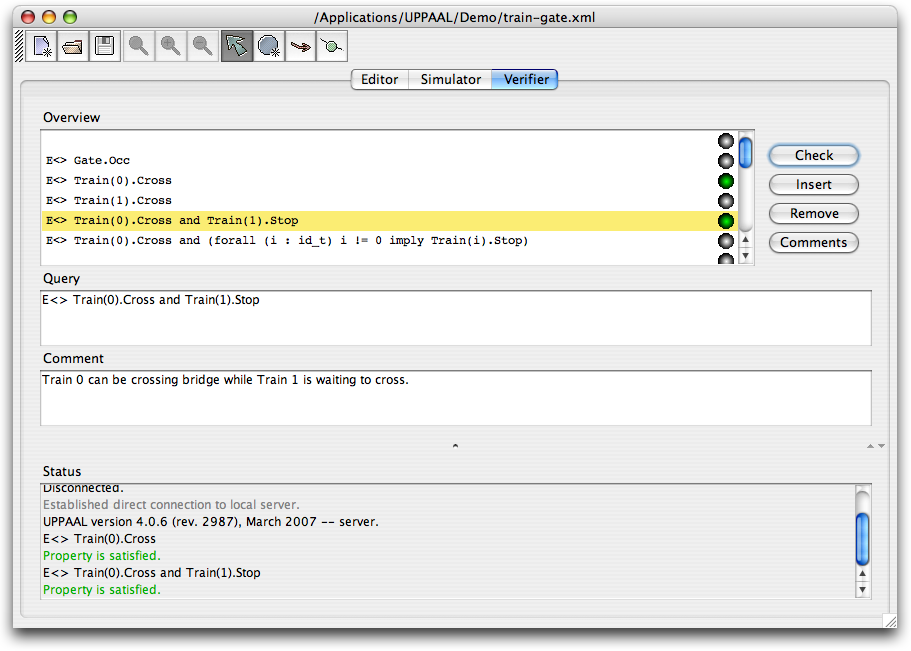
\includegraphics[width=\textwidth]{content/timed-automata/uppaal-3}
    \caption{UPPAAL: verification environment.}
    \label{fig:uppaal-3}
\end{figure}

Finally, the verification component (see Figure~\ref{fig:uppaal-3}) allows to perform model checking tasks by encoding requests in (timed) temporal logics. In fact, this component is directly using the command-line \emph{verifyta} tool to perform the verifications.

% ........................................................................... %

\chapter{UPPAAL and protocol timed automata}
\label{chap:uppaal-pta}

% ........................................................................... %

As we will see hereafter, checking emptiness on protocol timed automata with UPPAAL is not straightforward. We first explain the issues in converting a protocol timed automaton into an automaton that UPPAAL can process. We then propose a procedure for performing a semantic-preserving conversion. Finally, we illustrate it on the protocol $P_2'$ of Figure~\ref{fig:uppaal-pta}.\\

% ........................................................................... %

\section{Conversion issues}

% ........................................................................... %

We use UPPAAL for verifying whether a timed protocol is empty or not, i.e., whether it supports at least a conversation or not. To do that, we consider each final location of a protocol timed automaton and leverage UPPAAL to verify if it can be reached from its initial location or not (i.e., there exists a timed word whose execution over the protocol timed automaton ends in the considered final location). The language that is recognized by a protocol timed automaton is not empty as long as one final location can be reached.\\

This checking is however not straightforward. Indeed, a protocol timed automaton cannot be directly given to UPPAAL:
\begin{enumerate}
  
  \item clocks in UPPAAL are defined over $\Rpos$ whereas protocol timed automata are defined over $\Rpos \cup \{ \perp \}$, and
  
  \item in protocol timed automata, the clocks are initially set to $\perp$ and keep this value until they have been reset for the first time while in classical timed automata (and hence for UPPAAL) they start from 0 and immediately start their progression, and
  
  \item UPPAAL expects the guards to be conjunctions of atomic clock constraints (e.g., $x \:\#\; k$) and diagonal constraints (e.g., $x - y \;\#\; k$).
  
\end{enumerate}

% ........................................................................... %

\section{Conversion technique}

% ........................................................................... %

These differences can be overcome as UPPAAL does not work on \emph{strict} timed automata, but rather uses an hybrid model where non-clock variables can be defined, reset on switches and used in guards \cite{UPPAAL}. We propose the following procedure for checking protocol timed automata emptiness using UPPAAL. It has been implemented as part of the ServiceMosaic Protocols project presented earlier.

\begin{procedure}
Let us consider a protocol timed automaton $A$. The first step is to generate a UPPAAL model \texttt{Process} as follows.
\begin{enumerate}

	\item Remove the disjunctions in the guards of $A$:
	\begin{enumerate}
		\item obtain the abstract syntax tree (AST) of each constraint, then
		\item use an AST visitor \cite{Gamma95}: for each disjunction node, split into two switches (the disjunction node is replaced by the left-hand node in one switch guard, and by the right-hand node in the other switch guard)
		\item repeat until no AST contains a disjunction.
	\end{enumerate}
	
	\item Assign a unique boolean variable $b_x$ (initially set to \texttt{false}) to each switch that is set to \texttt{true} in the switch reset. This encodes $\perp$.
	
	\item Using an AST visitor, for each constraint clause $(x \;\#\; k)$ where $k \neq \perp$, rewrite as $(x \;\#\; k) \wedge (b_x = \mathtt{true})$ (note that it does not make sense to write a diagonal constraint comparing to $\perp$). When $k = \perp$, rewrite it as $(x \;\#\; k) \wedge (b_x = \mathtt{false})$.

\end{enumerate}

Finally, to check for emptiness: for each final location $l$, the corresponding TCTL property to be passed to UPPAAL is \texttt{E<> Process.l} and the procedure stops at the first final location $l$ such that the property is met, else the the timed language is empty.
\label{proc:emptiness}
\end{procedure}

We can point out the following remarks.
\begin{itemize}
  \item A procedure can be derived from this one to verify event-recording timed automata using UPPAAL.
  \item The procedure generates an automaton which is not a protocol timed automaton.
  \item Removing disjunctions from guards had already been discussed in \cite{BBVD+99} -- in fact the technique is the same.
\end{itemize}

% ........................................................................... %

\section{Sample conversion and emptiness checking}

% ........................................................................... %

\begin{figure}[htbp]
  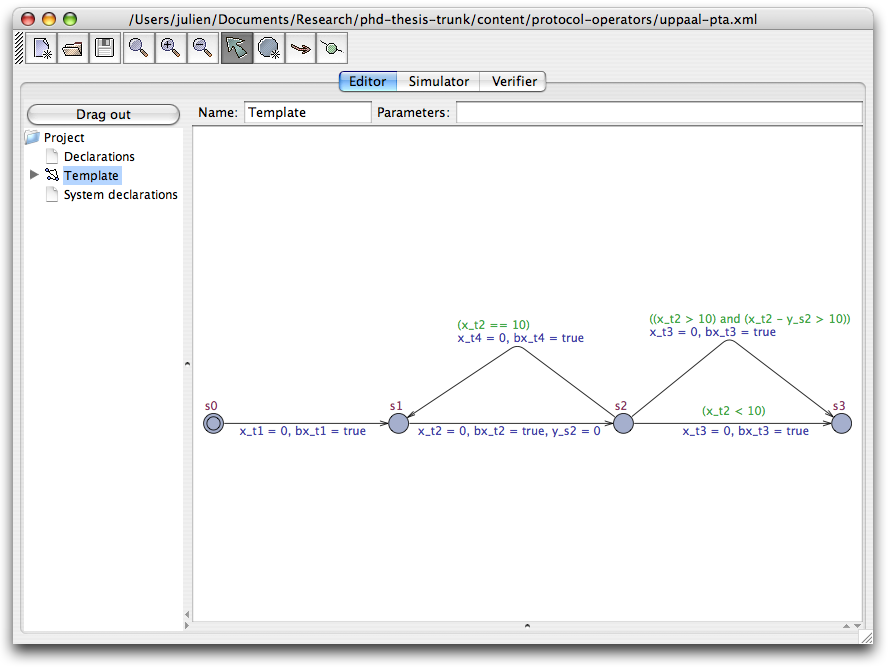
\includegraphics[width=\textwidth]{content/protocol-operators/uppaal-pta-1}
  \vspace{-0.5cm}
  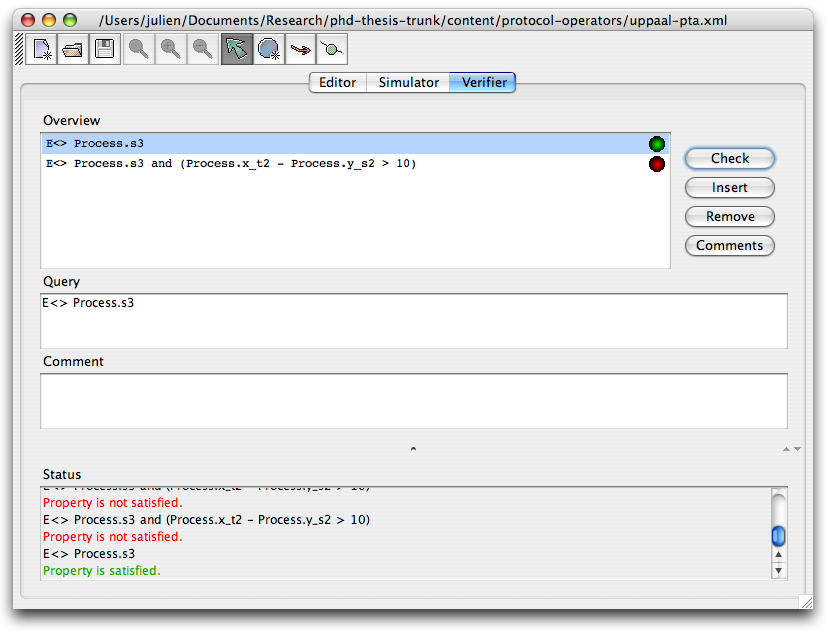
\includegraphics[width=\textwidth]{content/protocol-operators/uppaal-pta-2}
  \caption{Emptiness checking of protocol timed automata with UPPAAL.}
  \label{fig:uppaal-pta}
\end{figure}

Let us consider the protocol timed automaton $P_2$ of Figure~\ref{fig:sample-intersection}. The conversion to a UPPAAL automaton is illustrated on Figure~\ref{fig:uppaal-pta} along with the emptiness checking. As we can see, the conversion involves adding an extra switch between $S_2'$ and $S_3'$ as the permits clause is disjunctive and UPPAAL forbids disjunctions in guards.\\

The emptiness checking is performed using the following query:
$$ E\Diamond\; \mathtt{Process.s3} $$
On the figure, we have also added another query:
$$ E\Diamond\; \mathtt{Process.s3} \;\mathtt{and}\; (\mathtt{Process.x\_t2} - \mathtt{Process.y\_s2} > 10)$$
that checks that the $\varepsilon$-labeled switch is enforced. Indeed, due to the configuration of this automaton, the added switch with a guard \texttt{((x\_t2 > 10) and (x\_t2 - y\_s2 > 10))} cannot be taken under \MInvoke semantics.\\

Here is the corresponding UPPAAL automaton XML file:
{
  \footnotesize
  \verbatiminput{content/protocol-operators/uppaal-pta.xml}
}

Here is also the UPPAAL queries file:
{
  \footnotesize
  \verbatiminput{content/protocol-operators/uppaal-pta.q}
}

% ........................................................................... %